%csbd_acl

\documentclass[../../main/main.tex]{subfiles}

\begin{document}
\title{Certified Security by Design (CSBD) \& Access\-Control Logic (ACL)}

%%%%%%%%%%%%%%%%%%%%% Chapter CSBD ACL %%%%%%%%%%%%%%%
\chapter[Certified Security by Design (CSBD) \& Access-Control Logic (ACL)]{Certified Security by Design (CSBD)  \\ \& \\ Access-Control Logic (ACL)} \label{chp:csbdacl}


      %%%%%%%%%%%%%%%%%%% Section CSBD %%%%%%%%%%%%%%%%%%
\section{Certified Security by Design (CSBD)} \label{sec:csbd}

\begin{quote}
\textit{
"Providing satisfactory security controls in a computer system is in itself a system design problem."}  
\end{quote}

\begin{flushright}
Rand Corporation, 1970 \cite{defensescienceboard}
\end{flushright}

\glsentrylong{csbd} (\gls{csbd}) is a method for formally verifying and documenting the security properties of a systems.  It satisfies the principle of complete mediation.  It uses an access-control logic (ACL) to reason about access to security sensitive objects.  It uses computer-aided reasoning such as the Higher Order Logic (HOL) Interactive theorem prover to formally verify and document these security properties.  The outcomes of \gls{csbd} are consistent with the Systems Security Engineering (\gls{sse}) Framework described in \gls{nist} SP 800-160 \cite{NIST800160}.  They serve as a reproducible and auditable documentation of trustworthiness.

This chapter first describes \gls{csbd}'s access-control logic (\gls{acl}) used to prove complete mediation.  It then describes \gls{acl}'s implementation in the Higher Order Logic (\gls{hol}) Interactive Theorem prover.  Properties of transition systems are described in chapter \ref{chp:ssmmodel}.  The \gls{hol} code is included with this thesis in the foler /MasterThesis/HOL/ACL and pretty-printed code is included in appendix \ref{ppacl}.

      %%%%%%%%%%%%%%%%%%% Section ACL %%%%%%%%%%%%%%%%%%%
\section{Access-Control Logic (ACL)} \label{sec:acl}
The \gls{acl} is a logic for reasoning about security in the sense of \gls{cia}.  It develops formal proofs based on a formal prepositional logic to verify complete mediation.  This documentation is reproducible and is consistent with the SSE Framework.

\subsection{ACL: A Command and Control (C2) Calculus} \label{ssec:aclc2}
In the jargon of the day \gls{acl} is a command and control (C2) calculus with a set of axioms and logical rules used to reason about access-control.  At its most basic, the \gls{acl} is composed of principals that make requests to access objects.  These principals are given authority or jurisdiction over objects.  These principals must be authenticated before they can access or modify objects over which they have authority.  The following sections describe the components and logical rules of the \gls{acl}.

\subsection{Principals}\label{ssec:principals}
Principals should be thought of as actors in the access-control logic.  Principals can make statements or requests.  They can be assigned privileges or authority over objects or actions.  The text defines allowable principals using the identifier \textbf{Princ}:


\begin{center}
\textbf{Princ ::= PName / Princ \& Princ / Princ \textbar  Princ}\label{Princ}
\end{center}

This is a recursive definition. \textbf{\textit{PName}} refers to the name of a principal (i.e., Jane, PlatoonLeader, sensor1).  \textbf{\textit{Princ} \& \textit{Princ}} is read "Princ with Princ" or "Princ and Princ" (i.e., Principal1 with Principal2). \textbf{\textit{Princ \textbar  Princ}} is read as "Princ quoting Princ" (i.e., Principal1 quoting Principal2).


\subsection{Propositional Variables, Requests, Authority, Jurisdiction, and Delegation}\label{ssec:statementsacl}
To reason about access-control and trust, the \gls{acl} uses propositional variables, requests, authority, and jurisdiction to make statements.

Propositions in logic are assertions that are either true or false.  For example, "I am reading this master thesis" is a proposition because either you are or you are not reading this.  Propositional variables are just place holders for propositions.  For example, "I am reading this master thesis and doing something", where the propositional variable "doing something" could be replaced with "I am reading now" or "I am drinking coffee", etc..

Principals can make requests.  In the \gls{acl}, principals make requests using the \textit{says} operator.  Requests have the form \textit{P says $\varphi$},  where \textit{P} represents some principal and \textit{$\varphi$} represents some assertion (proposition, propositional variable).  For example, \textit{PlatoonLeader says platoonHalt}.  In this example, the Platoon Leader is issuing a command (or request) for the platoon to halt.  

Principals can have authority over assertions.  The \gls{acl}conveys authority using the \textit{controls} operator.  Statements of authority have the form \textit{P controls $\varphi$},  where \textit{P} represents some principal and \textit{$\varphi$} represents some assertion.  For example, \textit{PlatoonLeader controls platoonHalt}.  This states that the Platoon Leader has the authority over the command (or request) for the platoon to halt. 

Principals can also have jurisdiction over assertions.  Both authority and jurisdiction use the \textit{controls} operator.  Statements of jurisdiction have the same form as statements of authority.  Statements of authority are typically defined in an organization's policy.  Statements of jurisdiction are statements that are readily believed given the context.  For example, \textit{PresidentOfUS controls (PlatoonLeader controls platoonHalt)}.  In this example, the President of the United States, per the U.S. Constitution, has jurisdiction over the authority invested in the Platoon Leader.  In particular, the President of the United States has the jurisdiction to give the Platoon Leader the authority to command her platoon to halt.

In addition, principals can speak for other principals.  Principals do this using the \textit{speaks for} operator.  The ACL represents the \textit{speaks for} operator with the symbol $\Rightarrow$.  These types of statements have the form \textit{P $\Rightarrow$ Q}, where both \textit{P} and \textit{Q} are principals.  The \textit{speaks for} operator is typically used to reason about certifications issued by some authority.  For example, a driver's license speaks for the Department of Motor Vehicles.  

Principals can also delegate authority.  Principals do this using the \textit{reps} rule.  The \textit{reps} rule assigns authority given to one principal to another principal.  For example, the Platoon Leader \textit{reps} the President of the United States on platoon leading commands.

The concept of assigning integrity and security levels (such as classification) to principals and objects is also covered in the \gls{acl}.  But, they are not discussed in this master thesis because they are beyond the scope of this work.

\subsection{Well-formed Formulas}\label{ssec:wff}
\Glspl{wff} define the syntax (or grammatical structure) of the propositional logic.  They are valid statements in the \gls{acl}.  All \gls{acl} statements must be a \gls{wff}.  The text book defines the set of \gls{wff}s using the identifier \textbf{Form}:

\begin{center}\label{wffdef}
\textbf{Form} ::= \textbf{PropVar} / $\neg$ \textbf{Form} / (\textbf{Form} $\vee$ \textbf{Form}) / \\ 
	                  (\textbf{Form} $\wedge$ \textbf{Form}) / (\textbf{Form} $\supset$ \textbf{Form}) / (\textbf{Form} $\equiv$ \textbf{Form}) / \\
	                  (\textbf{Princ} $\Rightarrow$ \textbf{Princ}) / (\textbf{Princ} says \textbf{Form}) / (\textbf{Princ} controls \textbf{Form}) /\\
	                  (\textbf{Princ} reps \textbf{Princ} on \textbf{Form}\footnote{The last line is from \cite{certmanual}.})
\end{center}

This is a recursive definition.  \textbf{\textit{PropVar}} is a propositional variable.  The symbols $\neg$, $\vee$, $\wedge$, $\subset$, and $\equiv$ are the standard set and logical symbols.  They represent "not", "or", "and", "implication", and "equivalence", respectively.  

\subsection{Kripke Structures \& Semantics}\label{ssec:kripke}
Kripke structures are named after Saul Kripke.  Kripke is an influential figure in logic and philosophy.  He is recognized, in particular, for inventing the Kripke semantics for modal logic \cite{saulk}.    

Whereas \gls{wff}s define the syntax of the propositional logic, Kripke semantics describe the semantics.  Semantics refers to the meaning of statements. 

\subsubsection{Kripke Structures}
A Kripke structure primarily deals with three things: worlds, propositions, and principals.  The worlds can be thought of as possible states or configurations of some system.  Propositions are just statements that are either true or false.  And, principals are just actors.  A Kripke structure $\mathcal{M}$ = $\langle \textit{W}, \textit{I}, \textit{J} \rangle $  is defined as a three-tuple consisting of the following: a set of worlds \textit{W}; a function \textit{I} called the assignment function that maps propositions to worlds, and ; a function \textit{J} that maps principals to relations on worlds, where the relation is called the accessibility relation.  Formally, these are defined as follows (definition 2.1 in the text): 

\begin{itemize}
\item \textit{W is a nonempty set, whose elements are called worlds.}
\item \textit{$I: \mathbf{PropVar} \rightarrow \mathcal{P}(W)$ is an interpretation function that maps each propositional variable to a set of worlds.}
\item \textit{$J: \mathbf{PName} \rightarrow \mathcal{P}((W \times W)$ is a function that maps each principal name to a relation on worlds.}
\end{itemize}

One way to think of Kripke structures is as a logic on multiple worlds or possible states.  
%For example, consider two planets Earth and Tatooine\footnote{Tatooine is the fictional home planet of Luke Skywalker.  Tatooine has two suns.  \cite{Tantooine}}.  Let $\varphi$ be the proposition "this is planet Tatooine" and $\theta$ be the proposition "this is a planet."  Then $I(\varphi) = \{Tatooine\}$ and $I(\theta) = \{Earth, Tatooine\} = W$, where \textit{W} is the set of all worlds (\{Earth, Tatooine\}).  Furthermore, let "Luke" and "Lea" and "Uncle Owen" be principals.  Now consider the following:  Luke can get from Earth to Earth, from Tatooine to Tatooine, and from Tatooine to Earth (and vis-a-vis).  He can also get from Tatooine to Tatooine.  Lea can get from Earth to Earth and from Tatooine to Earth (and vis-a-vis).  But, she can not get from Tatooine to Tatooine.  Uncle Owen can only get from Tatooine to Tatooine.  He can not get to Earth.  Then, $J(Luke) = \{(Earth, Earth),(Earth, Tatooine),(Tatooine, Earth), (Tatooine, Tatooine)\}$.  $J(Lea) = \{(Earth, Earth),(Earth, Tatooine),(Tatooine, Earth)\}$. And, $J(Uncle Owen) = \{(Tatooine, Tatooine)\}$. With \textit{W}, \textit{J}, and \textit{I} defined, this forms a Kripke structure.
%
%
%
Kripke structures are necessary to define the ACL properly.  In particular, they are necessary to define the concepts of "satisfies" and "soundness" which follow.  However, an in-depth understanding of Kripke structures is not necessary to understand the work in this master thesis.  

\subsubsection{Kripke Semantics}\label{ssec:kripkesemantics}
The Kripke semantics define the meanings of \gls{wff}s for Kripke structures.  The semantics can be thought of as an evaluation function for a particular Kripke $\mathcal{M}$ = $\langle \textit{W}, \textit{I}, \textit{J} \rangle $.  Figure \ref{kripkesemantics} shows the Kripke semantics.  The subscript $\mathcal{M}$ signifies that the evaluation function is defined for a particular Kripke structure.  This means there is a separate evaluation function for each Kripke structure.


\begin{figure}[h]
\centering
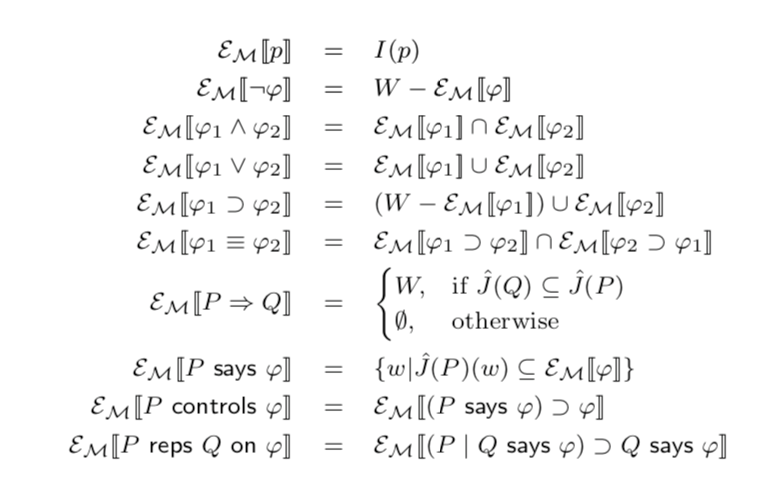
\includegraphics{../figures/kripkesemantics}
\caption{\label{kripkesemantics} Kripke semantics. Image taken from \textit{Access Control, Security, and Trust: A Logical Approach}\cite{ChinOlder}}
\end{figure}

%For example, for the Kripke structure described above, $\varepsilon_{\mathcal{M}}\textlbrackdbl \varphi \textrbrackdbl  = \{Tantooine\}$ and $\varepsilon_{\mathcal{M}}\textlbrackdbl \theta \textrbrackdbl  = \{Earth, Tantooine\} = W$ (the set of all worlds).  As an another example, $\varepsilon_{\mathcal{M}}\textlbrackdbl \text{Luke says $\varphi$} \textrbrackdbl = \{Earth, Tatooine\}$\footnote{Think about it.  }
%
\subsubsection{Satisfies}\label{sssec:satisfies}
The "satisfies" condition applies to a particular Kripke structure $\mathcal{M}$ = $\langle \textit{W}, \textit{I}, \textit{J} \rangle $.  It is said that $\mathcal{M}$ satisfies some proposition $\varphi$ if the evaluation function $\varepsilon_{\mathcal{M}}\textlbrackdbl \varphi \textrbrackdbl = W$ (the set of all worlds) for  $\mathcal{M}$.  In other words, $\varphi$ is true in all worlds of $\mathcal{M}$.  Symbolically, this is denoted as $\mathcal{M} \models \varphi$.  The statement $\mathcal{M}$ does not satisfy $\varphi$ is denoted as $\mathcal{M} \not\models \varphi$.

%In the example above, the Kripke structure $\mathcal{M} \models \theta$, where $\theta =$ the proposition "this is a planet."

\subsubsection{Soundness}\label{sssec:soundness}
Whereas "satisfies" describes a property of a Kripke structure $\mathcal{M}$, "soundness" describes a property of all Kripke structures. 

Soundness refers to the logical consistency of inference rules.  Inference rules consist of a set of hypothesis \{$H_1, H_2, \dots , H_n$\} and a conclusion. 
\begin{equation*}
\frac{H_1, H_2, \dots , H_n}{C}
\end{equation*}

An inferences rule is said to be sound if for every Kripke structure $\mathcal{M}$ that satisfies all the hypotheses, the conclusion is true. In other words,  the inference rule is sound if and only if $\forall H_i, \mathcal{M} \models H_i \longrightarrow \mathcal{M} \models C$.

Soundness is verified by formal proofs that employ axioms, tautologies, and sound inference rules that are already proved.  

\subsection{Inference Rules}\label{ssec:inferencerules}
The inference rules for the \gls{acl} are shown in figure \ref{inferencerules}.  All the inference rules are sound.  Details of proofs of soundness can be found in \textit{Access Control, Security, and Trust: A Logical Approach}\cite{ChinOlder}.

\begin{figure}[h]
\centering
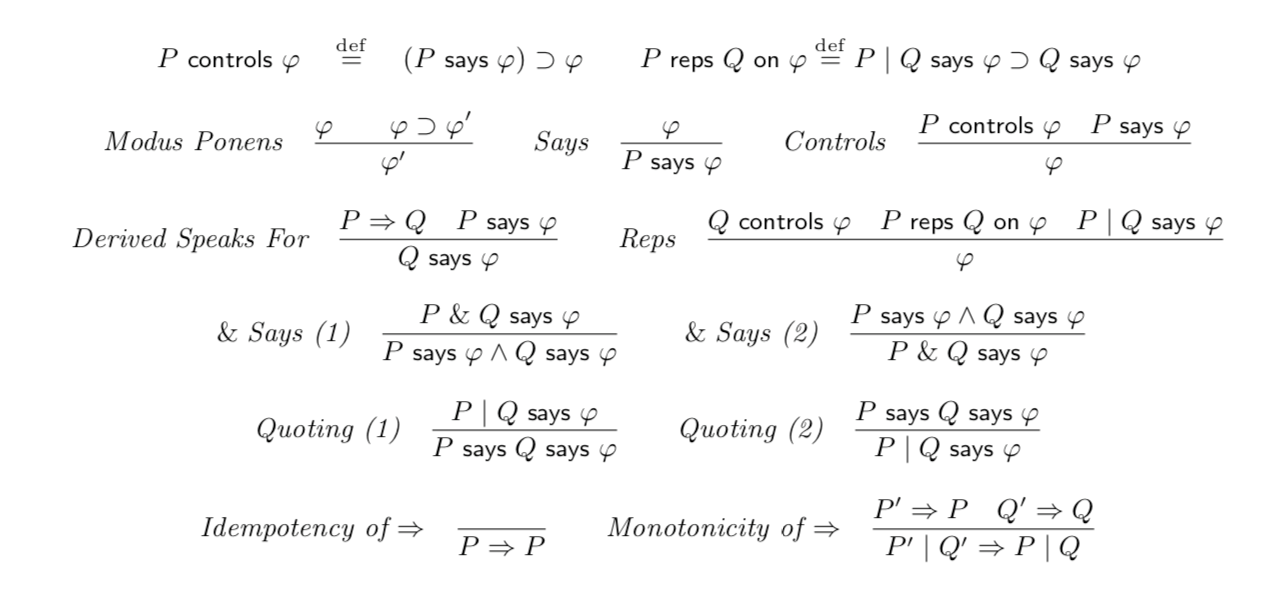
\includegraphics[width=\textwidth]{../figures/inferencerules}
\caption{\label{inferencerules}The \gls{acl} inference rules. Image taken from \textit{Access Control, Security, and Trust: A Logical Approach}\cite{ChinOlder}}
\end{figure}

\subsection{Complete mediation}\label{ssec:aclcompletemediation}
Fundamental to security is the concept of complete mediation.  This means that each principal must be authenticated and authorized on each request.   \gls{acl} does this primarily using the \textit{Controls} inference rule shown in figure \ref{inferencerules} and shown again here in figure \ref{ControlsInferenceRule}. 

\begin{figure}[h]
\centering
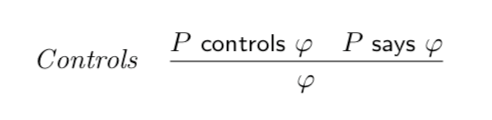
\includegraphics{../figures/ControlsInferenceRule}
\caption{\label{ControlsInferenceRule}The \textit{Controls} inference rule. Image taken from \textit{Access Control, Security, and Trust: A Logical Approach}\cite{ChinOlder}}
\end{figure}

This rule has two hypotheses and one conclusion. The left hypothesis is an authorization\footnote{or a \textit{control} in the C2 calculus}.  The principal P controls (is authorized on) some assertion $\varphi$. The right hypothesis is a request \footnote{or a \textit{command} in the C2 calculus}.  The principal P requests some assertion $\varphi$. The conjunction of the authorization and the request of P on $\varphi$ results in the assertion $\varphi$.  That is, if \textit{P controls $\varphi$} and\textit{ P says $\varphi$} then $\varphi$  is true.  

The \textit{Controls} rule is sufficient for basic authorization involving one principal and some assertion.  It is the only rule applied in this master thesis.  But, there are more complicated rules that allow for additional authentication and authorization schemes.  

\begin{figure}[h]
\centering
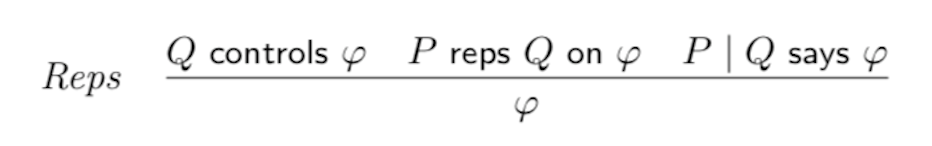
\includegraphics[width =0.7 \textwidth]{../figures/repsrule}
\caption{\label{repsrule}The \textit{Reps} inference rule. Image taken from \textit{Access Control, Security, and Trust: A Logical Approach}\cite{ChinOlder}}
\end{figure}

The \textit{Reps} (shown in figure \ref{repsrule}) rule also demonstrates complete mediation.  It follows a similar logic.  But, this rule has two principals, in this case P and Q.  The idea is that Q controls (is authorized on) some assertion $\varphi$. And also, P represents Q on that assertion.  In the \gls{acl}, this means that \textit{P Reps Q on $\varphi$}.  Note that \textit{P says $\varphi$} is not the same thing as \textit{P \textbar Q says $\varphi$} (short for, \textit{P says Q says $\varphi$}).  Spelled out, the rule follows as such: if \textit{Q controls $\varphi$ and P reps Q on $\varphi$ and P \textbar Q on $\varphi$} then $\varphi$ is true.

%The \textit{Reps} rule represents a principal acting in a role.  For example, soldier G.I. Jane may be acting as the Platoon Leader.  In this situation, it is the Platoon Leader (Q) who is granted authority over the command $\varphi$.  But, it is G.I.Jane (P) acting in the role of Platoon Leader who (Q) is actually issuing the command $\varphi$.  
%
\begin{figure}[h]
\centering
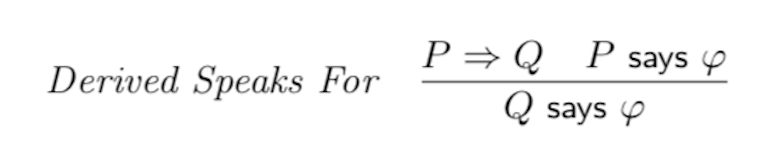
\includegraphics[width =0.6 \textwidth]{../figures/derivedspeaksfor}
\caption{\label{derivedspeaksfor}The \textit{Derived Speaks For} inference rule. Image taken from \textit{Access Control, Security, and Trust: A Logical Approach}\cite{ChinOlder}}
\end{figure}

The \textit{Derived Speaks For} rule usually applies to jurisdiction. This rule is shown in figure \ref{derivedspeaksfor}.  In this case, the principal P is "speaking for" the principal Q.  Again, the symbol $\Rightarrow$ means "speaks for."  Thus, if \textit{P $\Rightarrow$ Q and P says $\varphi$} then we believe that \textit{Q says $\varphi$}.

%The most common use of the \textit{Derived Speaks For}  rule is in jurisdictional case.  For example, the United States Army has jurisdiction over who serves in the role of Platoon Leader.  The U.S. Army may, in turn, issue i.d. cards with a soldier's photo (or in the future chips) that say, for example, soldier G.I.Jane is who the she says she is.  If we believe the i.d. card is genuine and it belongs to G.I.Jane, then the  i.d. card speaks for G.I.Jane.  So, if the i.d. card says issue G.I.Jane her equipment, then it follows that G.I. Jane says to issue her the equipment.  It is somewhat more complicated, because the U.S. Army has jurisdiction over who gets what equipment.  The i.d. card is not saying that G.I.Jane has control over her equipment.  It only says that she is asking for the equipment.  
%


      %%%%%%%%%%%%%%%%%%% Section ACL in HOL %%%%%%%%%%%%%%%
\section{ACL in HOL} \label{sec:aclinhol}
The material in this section is adapted from \textit{Access Control, Security, and Trust: A Logical Approach}\cite{ChinOlder} and \textit{Certified Security by Design Using Higher Order Logic}\cite{certmanual}. In this section, the former is referred to as "the text" and the later is referred to as "the manual."  


This section describes how the access-control logic (\gls{acl}) is implemented in the Higher Order Logic (\gls{hol}) Interactive Theorem Prover.  Pretty-printed \gls{hol}-generated output for all theories discussed in this section can be found in appendix \ref{ppacl}.  


\subsection{Principals}
Figure \ref{princHOL} shows the \gls{hol} representations for principals (\textbf{\textit{Princ}}).

\begin{figure}[h]
\centering
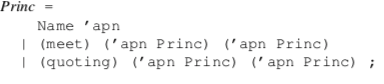
\includegraphics[width=0.6\textwidth]{../figures/princHOL}
\caption{\label{princHOL}The HOL implementation of principle (\textbf{\textit{Princ}}).  Image from  \textit{Certified Security by Design Using Higher Order Logic}\cite{certmanual}}.  
\end{figure}

 \textbf{\textit{Princ}} is an algebraic data type.  The concept of types are important in \gls{hol}.  They are discussed in the background chapter in section \ref{adt}. 

The definitions here correspond to the  \textbf{\textit{Princ}} defined in section \ref{Princ}.   The first line corresponds to \textbf{\textit{PropVar}}, the second corresponds to \textbf{Princ \& Princ}, and the third corresponds to \textbf{Princ \textbar  Princ}.  In \gls{hol} the infix \& operator is represented with the prefix \texttt{meet} operator.  The infix \textbar operator is represented with the prefix \texttt{quoting} operator.

%The primary difference between datatype definitions in \gls{hol} and ML (the metalanguage in which \gls{hol} is implemented) is that \gls{hol} does not use the keyword "of" before the type definition.  Thus, the first line of this definition is \texttt{Name 'apn} and not \texttt{Name of 'apn}.  As in ML, forward tick marks (apostrophes) always precede a type variable. 
%
Prefix operators may be used as infix operators if they are surrounded by a back tick \texttt{\textasciigrave} (typically located near the esc-key). This master thesis focuses on principals defined using the \texttt{Name PlatoonLeader} construction. 


In the definition for  \textbf{\textit{Princ}}, \texttt{Name} is called the type constructor.  The result of the constructor and a concrete type or type variable results in something of type \textbf{\textit{Princ}}.  Examples of principals in \gls{hol} are:
\[Name PlatoonLeader, or \]
\[(Name PlatoonLeader) \texttt{\textasciigrave} meet \texttt{\textasciigrave} (Name PlatoonSergeant), or \]
\[(Name PlatoonLeader) \texttt{\textasciigrave} quoting \texttt{\textasciigrave} (Name PlatoonSergeant). \]

\subsection{Well-Formed Formulas}
The \gls{hol} representation of \gls{wff}s is shown in figure \ref{FormACL}.

\begin{figure}[h]
\centering
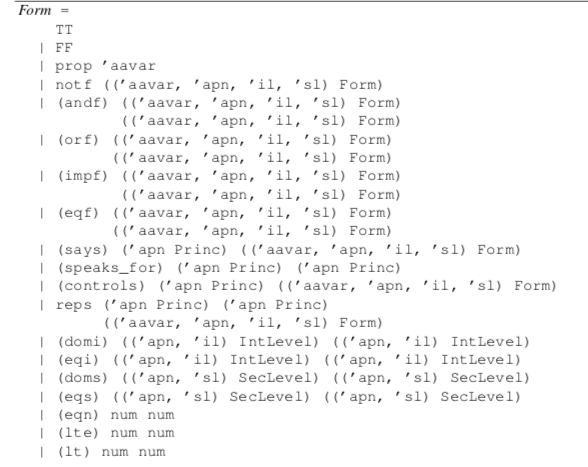
\includegraphics[width=\textwidth]{../figures/FormACL}
\caption{\label{FormACL}The definition for \textbf{Form} in \gls{hol}.   \textit{Certified Security by Design Using Higher Order Logic}\cite{certmanual}}
\end{figure}

\textbf{Form} is the datatype definition.  \texttt{TT}  and \texttt{FF} are the \gls{acl} representations of true and false, respectively.  \texttt{notf}, \texttt{andf}, \texttt{orf}, \texttt{impf}, \texttt{eqf}, \texttt{says}, \texttt{speaks_for}, \texttt{controls}, and \texttt{reps} are all the prefix version of the infix operators shown in the definition of \textbf{\textit{Form}} in section \ref{ssec:wff}.  The additional elements of the \textbf{Form} (from \texttt{domi} to the end) refer to integrity and security levels, which are not discussed in this master thesis. 

The type definitions that follow the operator are relevant and show-up everywhere in the code.  It is useful to dissect one of them.  Consider the \texttt{andf} operator.  
\[ \texttt{(andf) (('aavar, 'apn, 'il, 'sl) Form) }\]
\[ \texttt{(('aavar, 'apn, 'il, 'sl) Form)}. \]


\texttt{(('aavar, 'apn, 'il, 'sl) Form)} is the type signature for another \textbf{Form}.  The component types of a \textbf{Form} are a proposition (\texttt{'aavar}), a principal (\texttt{'apn}), an integrity level (\texttt{'il}), and a security level (\texttt{'sl}).  The prefix operator \texttt{andf} then takes two \textbf{Form}s each of type \texttt{(('aavar, 'apn, 'il, 'sl) Form)}.  
\subsection{Kripke structures}
Kripke structures are necessary to prove the ``satisfies" and ``soundness" properties of the \gls{acl}.   

%Therefore, they are only briefly described here. The \gls{hol} implementation of the Kripke structure is shown in figure \ref{kripkehol}.

\begin{figure}[h]
\centering
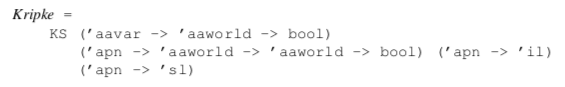
\includegraphics[width=1.0\textwidth]{../figures/kripkehol}
\caption{\label{kripkehol}The HOL implementation of a Kripke structure (\textbf{\textit{Princ}}).  Image from  \textit{Certified Security by Design Using Higher Order Logic}\cite{certmanual}}.  
\end{figure}

Kripke structures are defined previously as a three-tuple.  The Kripke structure here has four components (each surrounded by parentheses). This is different than what is described in section \ref{kripkesemantics}. 

In figure \ref{kripkehol}, the first set of parenthesis represents the assignment function more-or-less. It takes a proposition and world as arguments.  If the proposition is true in that world, then the function returns true, otherwise it returns false.  The second pair of parenthesis is similar to the accessibility function.  It takes a principal, a world, and another world.  The function returns true if the second world is accessible from the first for this particular principal, otherwise it returns false.  The last two pairs of parentheses represent integrity and security levels.  These are not discussed in this master thesis.  

The reader should recognize Kripke structures in the \gls{hol} code.  Kripke structures will either be fully typed or abbreviated.  These two forms are shown below, respectively.  
\[ (M, Oi, Os) \]
\[ \texttt{M:('prop, 'world,'pName, 'Int, 'Sec)Kripke, (Oi: 'Int po), (Os:'Sec po)} \]

The actual Kripke structure is represented by M and the integrity and security levels are represented by Oi and Os.  

\subsection{ACL Formulas}
It remains now to define the access-control logic (\gls{acl}) formulas in \gls{hol} specifically.  These are shown in figure \ref{aclformulasHOL}.

\begin{figure}[h]
\centering
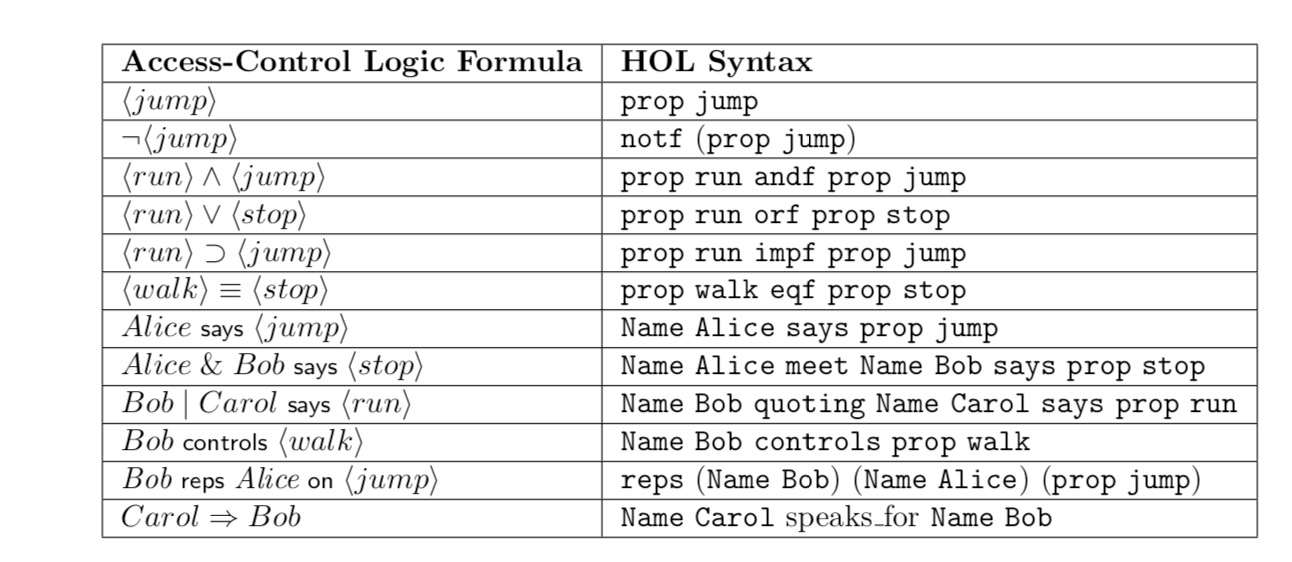
\includegraphics[width=\textwidth]{../figures/aclformulasHOL}
\caption{\label{aclformulasHOL}The \gls{acl} formulas in HOL.  Image taken from \textit{Access Control, Security, and Trust: A Logical Approach}\cite{ChinOlder}}
\end{figure}


Triangular brackets enclose propositions.  Thus, in the \gls{hol} representation of the \gls{acl}, a proposition is codes as follows:
\[\texttt{prop command} \]

A request in \glsentryshort{hol} is coded as: 
\[ \texttt{(Name PlatoonLeader) says (prop command)} \]

Parentheses are used when necessary\footnote{The need for parentheses is well-defined.  But, the author finds the best approach to parentheses is trial and error and generosity.}.  A statement of authority is coded as:
\[ \texttt{(Name PlatoonLeader) controls (prop command)} \]

These are the primary types of \gls{acl} formulas used in this master thesis.  The others are readily derivable from figure \ref{aclformulasHOL}.


\subsection{Kripke Semantics: The Evaluation Function}
The Kripke semantics described in section \ref{ssec:kripkesemantics} and shown in figure \ref{kripkesemantics} are also implemented in \gls{hol}.  This function is lengthy and the details are beyond the scope of this master thesis.  Part of the definition is shown \ref{Efn}.  The entire function can be found in appendix \ref{ppacl} in the section on aclsemantics.  The reader should note that the definition is defined for all Kripke structures as \texttt{$\forall$ Oi Os M}.


\begin{figure}[h]
\centering
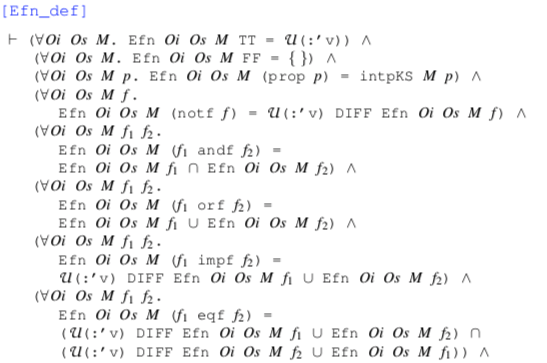
\includegraphics[width=\textwidth]{../figures/Efn}
\caption{\label{Efn}The \gls{hol} implementation of the Kripke semantics (evaluation function).  Image from  \textit{Certified Security by Design Using Higher Order Logic}\cite{certmanual}}
\end{figure}


\subsection{Satisfies And Soundness}
The implementation of the "satisfies" property is shown in figure \ref{satdef}.  Satisfies in this implementation is the same as soundness.
\begin{figure}[h]
\centering
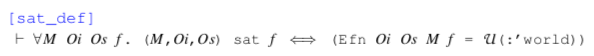
\includegraphics[width=\textwidth]{../figures/satdef}
\caption{\label{satdef}The \gls{hol} implementation of the "satisfies" property.  Image from  \textit{Certified Security by Design Using Higher Order Logic}\cite{certmanual}}
\end{figure}

The definition reads "f is true for the Kripke structure if and only if f for this Kripke structure it evaluates to all worlds.  The fact that is is defined for all Kripke structures \texttt{$\forall$ M Oi Os}. makes it sound.  

%
%The first part of the definition is \texttt{$\forall$ M Oi Os}.. This is the universal quantifier applied to all Kripke structure, integrity levels, security levels, and functions.   The next part of the definition is \texttt{(M, Oi, Os) sat f}.  This can read as "Kripke structure satisfied function f.'  The final part of the definition is \texttt{(Efn Oi Os M f = $\mathpzc{U}$(:'world))}.  This part states that the function \texttt{f} must evaluate to all worlds $\mathpzc{U}$.

%\subsection{Soundness}
%The definition for ``satisfies" in the \gls{hol} is similar to the definition for "soundness" described in section \ref{sssec:soundness}.  It can be read as "for all Kripke structures, the Kripke structure satisfies the function f 
%
%then the Kripke Structure is  In that section and the section preceding it, "satisfies" applied to a particular Kripke structure.  But, definition for ``satisfies" above is valid for all Kripke structures.  To extend this to ``soundness" it is only necessary to account for multiple hypotheses.  This is of the form shown in figure \ref{soundhol}
%
%
%\begin{figure}[h]
%\centering
%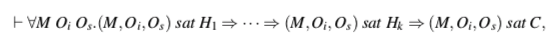
\includegraphics[width=\textwidth]{../figures/soundhol}
%\caption{\label{soundhol}The \gls{hol} representation of the ``soundness" property.  Image from  \textit{Certified Security by Design Using Higher Order Logic}\cite{certmanual}}
%\end{figure}
%
%A thorough description of the \gls{acl} in its entirety is beyond the scope of this master thesis.  All the theory files necessary to use this \gls{hol} implementation of the \gls{acl} are included with the files with this master thesis.  A pretty-printed EmitTeX version of the code is included in appendix \ref{ppacl}.  

The next chapter describes the patrol base operations as a modularized hierarchy of secure state machines.

\end{document}
